%%%%%%%%%%%%%%%%%%%%%%%%%%%%%%%%%%%%%%%%%
% Short Sectioned Assignment LaTeX Template Version 1.0 (5/5/12)
% This template has been downloaded from: http://www.LaTeXTemplates.com
% Original author:  Frits Wenneker (http://www.howtotex.com)
% License: CC BY-NC-SA 3.0 (http://creativecommons.org/licenses/by-nc-sa/3.0/)
%%%%%%%%%%%%%%%%%%%%%%%%%%%%%%%%%%%%%%%%%

%----------------------------------------------------------------------------------------
%	PACKAGES AND OTHER DOCUMENT CONFIGURATIONS
%----------------------------------------------------------------------------------------

\documentclass[paper=a4, fontsize=11pt]{scrartcl} % A4 paper and 11pt font size

% ---- Entrada y salida de texto -----

\usepackage[T1]{fontenc} % Use 8-bit encoding that has 256 glyphs
\usepackage[utf8]{inputenc}
%\usepackage{fourier} % Use the Adobe Utopia font for the document - comment this line to return to the LaTeX default

% ---- Idioma --------

\usepackage[spanish, es-tabla]{babel} % Selecciona el español para palabras introducidas automáticamente, p.ej. "septiembre" en la fecha y especifica que se use la palabra Tabla en vez de Cuadro

% ---- Otros paquetes ----

\usepackage{url} % ,href} %para incluir URLs e hipervínculos dentro del texto (aunque hay que instalar href)
\usepackage{amsmath,amsfonts,amsthm} % Math packages
%\usepackage{graphics,graphicx, floatrow} %para incluir imágenes y notas en las imágenes
\usepackage{graphics,graphicx, float} %para incluir imágenes y colocarlas

% Para hacer tablas comlejas
%\usepackage{multirow}
%\usepackage{threeparttable}

%\usepackage{sectsty} % Allows customizing section commands
%\allsectionsfont{\centering \normalfont\scshape} % Make all sections centered, the default font and small caps

\usepackage{fancyhdr} % Custom headers and footers
\pagestyle{fancyplain} % Makes all pages in the document conform to the custom headers and footers
\fancyhead{} % No page header - if you want one, create it in the same way as the footers below
\fancyfoot[L]{} % Empty left footer
\fancyfoot[C]{} % Empty center footer
\fancyfoot[R]{\thepage} % Page numbering for right footer
\renewcommand{\headrulewidth}{0pt} % Remove header underlines
\renewcommand{\footrulewidth}{0pt} % Remove footer underlines
\setlength{\headheight}{13.6pt} % Customize the height of the header

\numberwithin{equation}{section} % Number equations within sections (i.e. 1.1, 1.2, 2.1, 2.2 instead of 1, 2, 3, 4)
\numberwithin{figure}{section} % Number figures within sections (i.e. 1.1, 1.2, 2.1, 2.2 instead of 1, 2, 3, 4)
\numberwithin{table}{section} % Number tables within sections (i.e. 1.1, 1.2, 2.1, 2.2 instead of 1, 2, 3, 4)

\setlength\parindent{0pt} % Removes all indentation from paragraphs - comment this line for an assignment with lots of text

\newcommand{\horrule}[1]{\rule{\linewidth}{#1}} % Create horizontal rule command with 1 argument of height

\graphicspath{ {./images/} }
\usepackage{subcaption}
\usepackage{hyperref}
\usepackage{soul}


%----------------------------------------------------------------------------------------
%	TÍTULO Y DATOS DEL ALUMNO
%----------------------------------------------------------------------------------------

\title{	
\normalfont \normalsize 
\textsc{\textbf{Aprendizaje Automático (2019)} \\ Doble Grado en Ingeniería Informática y Matemáticas \\ Universidad de Granada} \\ [25pt] % Your university, school and/or department name(s)
\horrule{0.5pt} \\[0.4cm] % Thin top horizontal rule
\huge Proyecto Final \\ % The assignment title
\horrule{2pt} \\[0.5cm] % Thick bottom horizontal rule
}

\author{Ignacio Aguilera Martos, Luis Balderas Ruiz \\ \texttt{nacheteam@correo.ugr.es, luisbalderas@correo.ugr.es}} 
 % Nombre y apellidos 


\date{\normalsize\today} % Incluye la fecha actual

%----------------------------------------------------------------------------------------
% DOCUMENTO
%----------------------------------------------------------------------------------------

\begin{document}

\maketitle % Muestra el Título

\newpage %inserta un salto de página

\tableofcontents % para generar el índice de contenidos

\listoffigures

\listoftables

\newpage


%----------------------------------------------------------------------------------------
%	Introducción
%----------------------------------------------------------------------------------------

\section{APS Failure Scania Trucks Classification}

\subsection{Introducción}

Nos encontramos ante un problema de clasificación binaria (clase positiva y negativa) en la que la clase positiva consiste en el fallo o mal funcionamiento de un componente específico del sistema APS para la compañía de camiones Scania. Por su parte, la clase negativa está formada por camiones con fallos en componentes que no están relacionado con el sistema APS. En lo que se refiere al dataset en sí, el conjunto de entrenamiento está formado por 60000 instancias y 171 características. El test tiene 16000 muestras. Sabemos que los nombres de los atributos han sido anonimizados por motivos de privacidad. En el presente documento explicamos con detalle cada uno de los pasos que hemos seguido en el estudio y diseño de un sistema inteligente para la clasificación con varios modelos, a saber, un modelo lineal (SGD), una Máquina de Soporte de Vectores, un modelo basado en Boosting (AdaBoost, concretamente) y Random Forest. Previo uso de los modelos, hemos hecho un profundo estudio de los datos que nos han llevado a modificarlos y tratarlos para mejorar los resultados, entre lo que destaca el tratamiento de valores perdidos con la imputación de la mediana, eliminación de estancias poco relevantes, oversampling con SMOTE para compensar el gran desbalanceo y análisis factorial para reducir la dimensionalidad en las características. 

\section{Preprocesamiento}

\subsection{Análisis explotario y valores perdidos}

Nos encontramos ante un problema que tiene una gran cantidad de datos. En principio, este hecho es una ventaja, dado que la capacidad de generalización aumenta enormemente. Sin embargo, uno de los grandes retos ha sido, por un lado, el gran desbalanceo entre las clases y, por otro, la gran cantidad de valores perdidos e inconsistencias en los datos. Nos ocupamos de esto segundo en primer lugar. El análisis exploratorio de los datos nos hizo llegar a la conclusión de que, de entre las pocas instancias que forman parte de la clase positiva (esto es, con un fallo en el sistema APS), los valores de las variables estaban extraviados o, si no era así, más parecían outliers que otra cosa. En seguida nos dimos cuenta de que, desde un punto de vista físico tiene sentido, dado que la avería en un componente puede hacer que el comportamiento en los demás sea errático y, como consecuencia, puede generar observaciones de lo más variopintas. No obstante, nos dedicamos a eliminar los valores perdidos y le dimos validez total a los datos de los que disponemos. \\

En primer, vimos que había características que tenían más de un 70\% de sus valores como NA. Decidimos eliminarlas, ya que iban a entorpecer enormemente el trabajo de los modelos (en alguno de ellos, incluso son incompatibles). Eliminamos por tanto las características 2,75,76,77,78,79 y 113, por lo que pasamos de 171 a 164. En lo que se refiere a instancias, observamos que gran cantidad de ellas también estaban pobladas de valores perdidos. Teniendo en cuenta el gran desbalanceo de las clases, eliminamos aquellas instancias con etiqueta negativa que tuvieran más de un 15\% de sus entradas como NA, de forma que pasamos de 60000 instancias a 55964. \\

A partir de ahí, nuestro conjunto de datos es más tratable. Sin embargo, aunque más dispersos, aún hay muchos valores perdidos con los que los modelos no pueden lidiar. Para solucionarlo, consultando la bibliografía, utilizamos dos tipos de imputación de valores perdidos: imputación de la mediana y de la media. La mediana nos ha dado mejores resultados en general, por lo que continuamos nuestro desarrollo con la mediana. 

\subsubsection{Desbalanceo de clases}

Sin duda alguna, uno de los grandes problemas a los que nos enfrentamos cuando tratamos este conjunto de datos es el gran desbalanceo entre las clases. Hicimos una primera visualización de los datos observando el desbalanceo pero, a su vez, leve solapamiento (lo que a priori es una ventaja).

\begin{figure}[H] %con el [H] le obligamos a situar aquí la figura
		\centering
		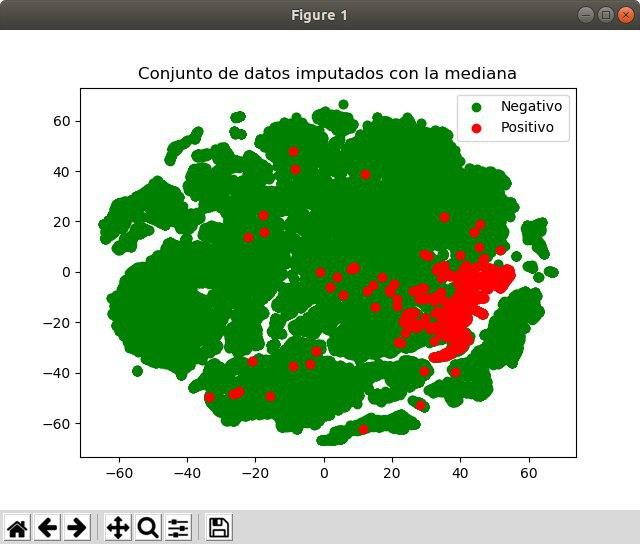
\includegraphics[scale=0.6]{pre-smote.jpg}  %el parámetro scale permite agrandar o achicar la imagen. En el nombre de archivo puede especificar directorios
		\caption{Representación de las instancias tras la imputación de VP con la mediana} 
	\label{fig:sep-clases}
\end{figure}

Sin embargo, a pesar de la separación de las clases éramos incapaces de generar buenos resultados con los modelos y los clasificadores siempre etiquetaban las instancias de test como pertenecientes a la clase negativa. Esto daba lugar a un buen accuracy, pero las demás medidas que tenemos en cuenta, como son recall o f1-score eran nefastas.

\begin{figure}[H] %con el [H] le obligamos a situar aquí la figura
	\centering
	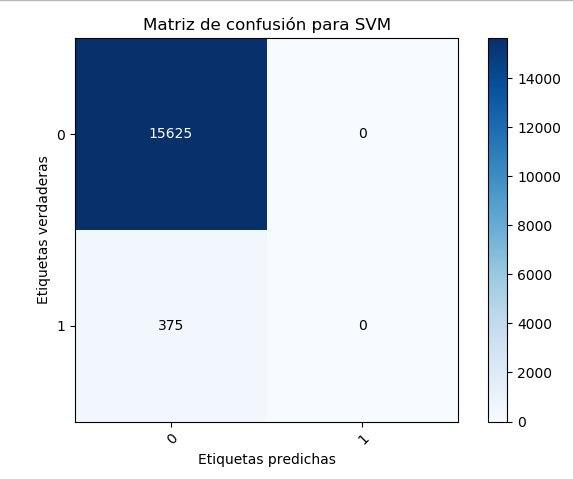
\includegraphics[scale=0.6]{conf1.jpg}  %el parámetro scale permite agrandar o achicar la imagen. En el nombre de archivo puede especificar directorios
	\caption{Matriz de confusión generada por SVM /RF/SGD/Red Neuronal hasta el momento} 
	\label{fig:conf1}
\end{figure}

Por tanto, a pesar de la buena disposición de los datos, no se obtenían buenos resultados. A la vista de los mismos, nos decantamos por utilizar técnicas de oversampling para equilibrar el número de instancias de cada clase. En particular, elegimos SMOTE (\cite{smote}) como herramienta. Tras su aplicación, contamos finalmente con 109928 instancias de cada clase, apareciendo la siguiente disposición de datos:

\begin{figure}[H] %con el [H] le obligamos a situar aquí la figura
	\centering
	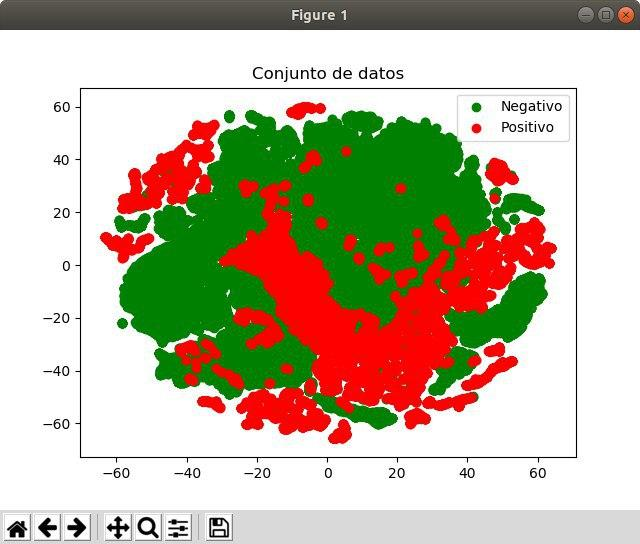
\includegraphics[scale=0.55]{tras-smote.jpg}  %el parámetro scale permite agrandar o achicar la imagen. En el nombre de archivo puede especificar directorios
	\caption{Disposición del dataset tras SMOTE} 
	\label{fig:post-smote}
\end{figure}

Como se puede apreciar, hemos perdido la localidad de las clases, aunque, como se verá, va a ser muy positivo.

\subsubsection{Selección de características}

Tras la eliminación de características por poseer demasiados valores perdidos, poseemos 164. No nos parece un número adecuado para utilizar PCA (más recomendado para cuando hay muchas más variables, ya que el sacrificio de la interpretabilidad es menos costoso) así que nos decantamos por otras técnicas de estadística multivariante, como es análisis factorial (\cite{ms},\cite{amsa},\cite{fa1}, \cite{fa2}). Análisis factorial sí nos ayuda a darle interpretabilidad al modelo y a encontrar qué características son las más determinantes. Reducimos así de 164 a 151. Sin embargo, los resultados en los modelos nos harán comprobar que, a pesar de mejorar el accuracy, se empeora la clasificación de las instancias de la clase positiva, como se puede ver en la siguiente comparación entre matrices de confunsión para Random Forest:

\begin{table}[H]
	\centering
	\begin{tabular}{|c|c|c|}
		\hline
		Verd \textbackslash Pred & 0     & 1    \\ \hline
		0                        & 56160 & 2840 \\ \hline
		1                        & 77    & 923  \\ \hline
	\end{tabular}
	\caption{Matriz de confusión sin FA}
\end{table}

\begin{table}[H]
	\centering
	\begin{tabular}{|c|c|c|}
		\hline
		Verd \textbackslash Pred & 0     & 1    \\ \hline
		0                        & 57077 & 1923 \\ \hline
		1                        & 113   & 887  \\ \hline
	\end{tabular}
	\caption{Matriz de confusión con FA}
\end{table}

Por tanto, como nuestro objetivo es maximizar todas las medidas, especialmente recall (la clase minoritaria sigue siendo, de forma natural, la clase positiva), optamos por no aplicar de forma definitiva análisis factorial. Después de explorar estas dos técnicas, llegamos a la conclusión de que el tamaño del dataset hace que el número de características no sea muy elevado, por lo que acabamos por no seleccionar ningún subconjunto de ellas.

\subsubsection{Normalización}

En el análisis exploratorio observamos que el rango de las variables es absolutamente dispar. Todos los clasificadores basados en instancias (que incorporan la distancia) necesitan de un rango de variables equivalente para poder dar el peso adecuada a cada una. Por eso, realizamos una normalización estándar a los datos.

 

%\begin{figure}[H] %con el [H] le obligamos a situar aquí la figura
%	\centering
%	\includegraphics[scale=0.6]{count-clases.png}  %el parámetro scale permite agrandar o achicar la imagen. En el nombre de archivo puede especificar directorios
%	\caption{Histograma con el número de instancias por clase} 
%	\label{fig:clases}
%\end{figure}


\newpage
\section{Bibliografía}

%------------------------------------------------

\bibliography{citas} %archivo citas.bib que contiene las entradas 
\bibliographystyle{plain} % hay varias formas de citar

\end{document}
